% 第三章 任意构型 Hopfion 的理论模型与构建
\chapter{任意构型 Hopfion 的理论模型与程序化构建}

\section{引言}

在研究磁性 Hopfion 的稳定性与动力学性质时，构建高质量的初始磁化分布是微磁学模拟的基础。前人提出的解析解（如 Sutcliffe 模型）能够为特定拓扑荷（如 $Q_H=1$）的 Hopfion 提供良好的初始状态，而在研究更高阶拓扑荷或不同空间取向的复杂构型时，已有学者提出了基于环面坐标系的理论模型\cite{guslienko2025magnetic}。本文并未提出新的理论解析解，而是基于前人成熟的局域旋转矩阵与环面坐标系映射理论，将这些纯数学的物理描述转化为可直接用于微磁学模拟的代码工具。本章主要介绍如何基于现有理论编写支持任意拓扑荷及反铁磁（AFM）背景交替的初始态结构生成脚本，并介绍了相关的三维可视化解调方法，为后续的仿真研究奠定基础。

\section{Hopfion 理论模型回顾}

\subsection{磁化场的旋转矩阵表示}
根据连续场理论，Hopfion 可以被视为嵌入在均匀磁化背景中的三维拓扑孤子。若设均匀背景磁化为 $\mathbf{m}_0 = \hat{z}$，任意复杂磁化构型 $\mathbf{m}(\mathbf{r})$ 可通过一个坐标依赖的局部旋转矩阵 $\hat{R}(\mathbf{r})$ 作用于背景得到，即 $\mathbf{m}(\mathbf{r}) = \hat{R}(\mathbf{r}) \mathbf{m}_0$。

引入超球面 $S^3$ 的四元数参数化向量 $n_\alpha = (n_1, n_2, n_3, n_4)$，其满足归一化条件 $\sum n_\alpha^2 = 1$。局部旋转矩阵可由 $n_\alpha$ 的分量构建：
\begin{equation}
    R_{ik} = \delta_{ik} + 2(n_i n_k - n^2 \delta_{ik}) - 2\varepsilon_{ikl} n_l n_4
\end{equation}
其中，下标 $i, k, l \in \{1,2,3\}$，$\mathbf{n} = (n_1, n_2, n_3)$，$n^2 = n_1^2 + n_2^2 + n_3^2$，$\varepsilon_{ikl}$ 为完全反对称张量。由此，三维空间中的磁化场分量可化简写为：
\begin{equation}
    \mathbf{m} = (1 - 2n^2)\hat{z} + 2n_z \mathbf{n} + 2n_4(\mathbf{n} \times \hat{z})
    \label{eq:hopf_magnetization}
\end{equation}

\subsection{环面坐标下的参数化}
在直角坐标系 $(x,y,z)$ 下直接描述 Hopfion 的核心形貌较为复杂。通过引入环面坐标系 $(\eta, \beta, \phi)$，可自然地将 $R^3$ 空间与超球面 $S^3$ 建立映射。直角坐标与环面坐标的转换关系为：
\begin{equation}
    \rho = \frac{a \sinh \eta}{\tau}, \quad z = \frac{a \sin \beta}{\tau}, \quad \phi = \arctan(y/x)
\end{equation}
其中 $\rho = \sqrt{x^2+y^2}$，$\tau = \cosh \eta - \cos \beta$，$a$ 为 Hopfion 核心环（$m_z=-1$ 所在的圆环）的特征大半径。

在该坐标系下，为了满足非平凡的 Hopf 映射，定义如下复函数形式：
\begin{align}
    Z_1 &= n_4 - i n_3 = e^{-im\beta} \cos \zeta(\eta) \\
    Z_2 &= n_2 - i n_1 = e^{in\phi} \sin \zeta(\eta)
\end{align}
结合公式~\eqref{eq:hopf_magnetization}，磁化矢量的面外（$z$）和面内（$x-y$）分量可化简为：
\begin{align}
    m_z(\eta, \beta, \phi) &= \cos(2\zeta(\eta)) \\
    m_x + i m_y &= \sin(2\zeta(\eta)) e^{i(n\phi + m\beta)}
\end{align}
其中，整数 $p=m$ 和 $q=n$ 分别代表极向（Poloidal）和方位向（Azimuthal）的缠绕数，系统的总 Hopf 指数为两者之积 $Q_H = p \times q$。函数 $\zeta(\eta)$ 定义了从核心到边界的衰减分布，需满足特定的边界条件，从而控制磁化在中心区域和无穷远处的渐进行为。这些前人建立的理论模型成功将复杂拓扑构型的描述转化为简单的整数参数设置。在理解并提取这些核心数学公式的基础上，本文接下来的主要工作是将其进行三维空间的离散化编程实现。

\section{离散化生成脚本与反铁磁拓展}

\subsection{程序化离散与网格构建}
基于上述解析理论，本文使用 Python 语言开发了磁化场初始态生成程序（见附录或代码库 \texttt{create\_hopfion\_AFM\_v2.py}）。该脚本首先在给定的三维计算空间内划分均匀的离散网格，得到三维坐标矩阵 $(x_i, y_j, z_k)$。通过中心偏移和平移操作后，将直角坐标转换为有效的局部环面坐标系统，进而计算每一个网格点处对应的磁化分量 $\mathbf{m}(x_i, y_j, z_k)$。

程序支持通过设置参数改变 Hopfion 核心环所在的平面（如由默认的 $x-y$ 平面切换至 $x-z$ 或 $y-z$ 平面），通过有效的坐标轮换变换，实现了拓扑结构在不同维度的灵活旋转，满足后续驱动实验中对特定初始磁化位向和传播方向的需求。计算完成的磁化数据最终导出为标准的 OOMMF OVF 2.0 二进制文件，可以直接被 Mumax3 等微磁学模拟软件作为初始态加载。

\subsection{反铁磁交替背景}
针对近期的研究热点——受挫磁体与具有反铁磁交换作用的复杂磁体系，生成脚本还引入了自适应的反铁磁（AFM）背景生成功能。通过在不同的空间维度上叠加符号交替矩阵（如三维 checkerboard 棋盘格模式，或针对特定轴向的 layer 分层模式），程序能够为生成的纯铁磁 Hopfion 附加不同样式的反铁磁序背景。此外，通过设置 \texttt{afm\_outside\_only} 参数，可将交替扰动严格限制在 Hopfion 核心区域之外，或实现全局交错。

\section{Hopfion 构型的可视化}

为验证构造算法的正确性并直观展示三维拓扑特征，本文进一步编写了基于等值面提取和三维渲染的可视化分析脚本（\texttt{draw\_afm\_new.py}）。

该脚本利用 Marching Cubes 算法从离散的网格数据中提取出 $m_z=0$ 的三维等值面，并根据该面上的面内磁化相位角 $\Phi = \arctan(m_y/m_x)$ 为其顶点赋予相应的颜色值。在此基础上，通过色相映射（Hue Map），可以在几何面片上清晰地观察到磁化矢量的连续扭转。

值得一提的是，针对包含 AFM 交替背景的结构文件，由于网格级的正负交替会导致等值面提取失效，可视化脚本中内嵌了自动信号解调（Demodulation）功能。算法首先通过计算相邻格点的平均点积，识别出反铁磁的分布模式与相位偏移，然后在提取等值面之前对局部反向磁矩进行预先翻转，将其“解调”回连续的铁磁场形式，从而成功实现等值面渲染并提取核心大半径 $R$ 和小半径 $r$。

\begin{figure}[htbp]
    \centering
    \begin{minipage}{0.48\textwidth}
        \centering
        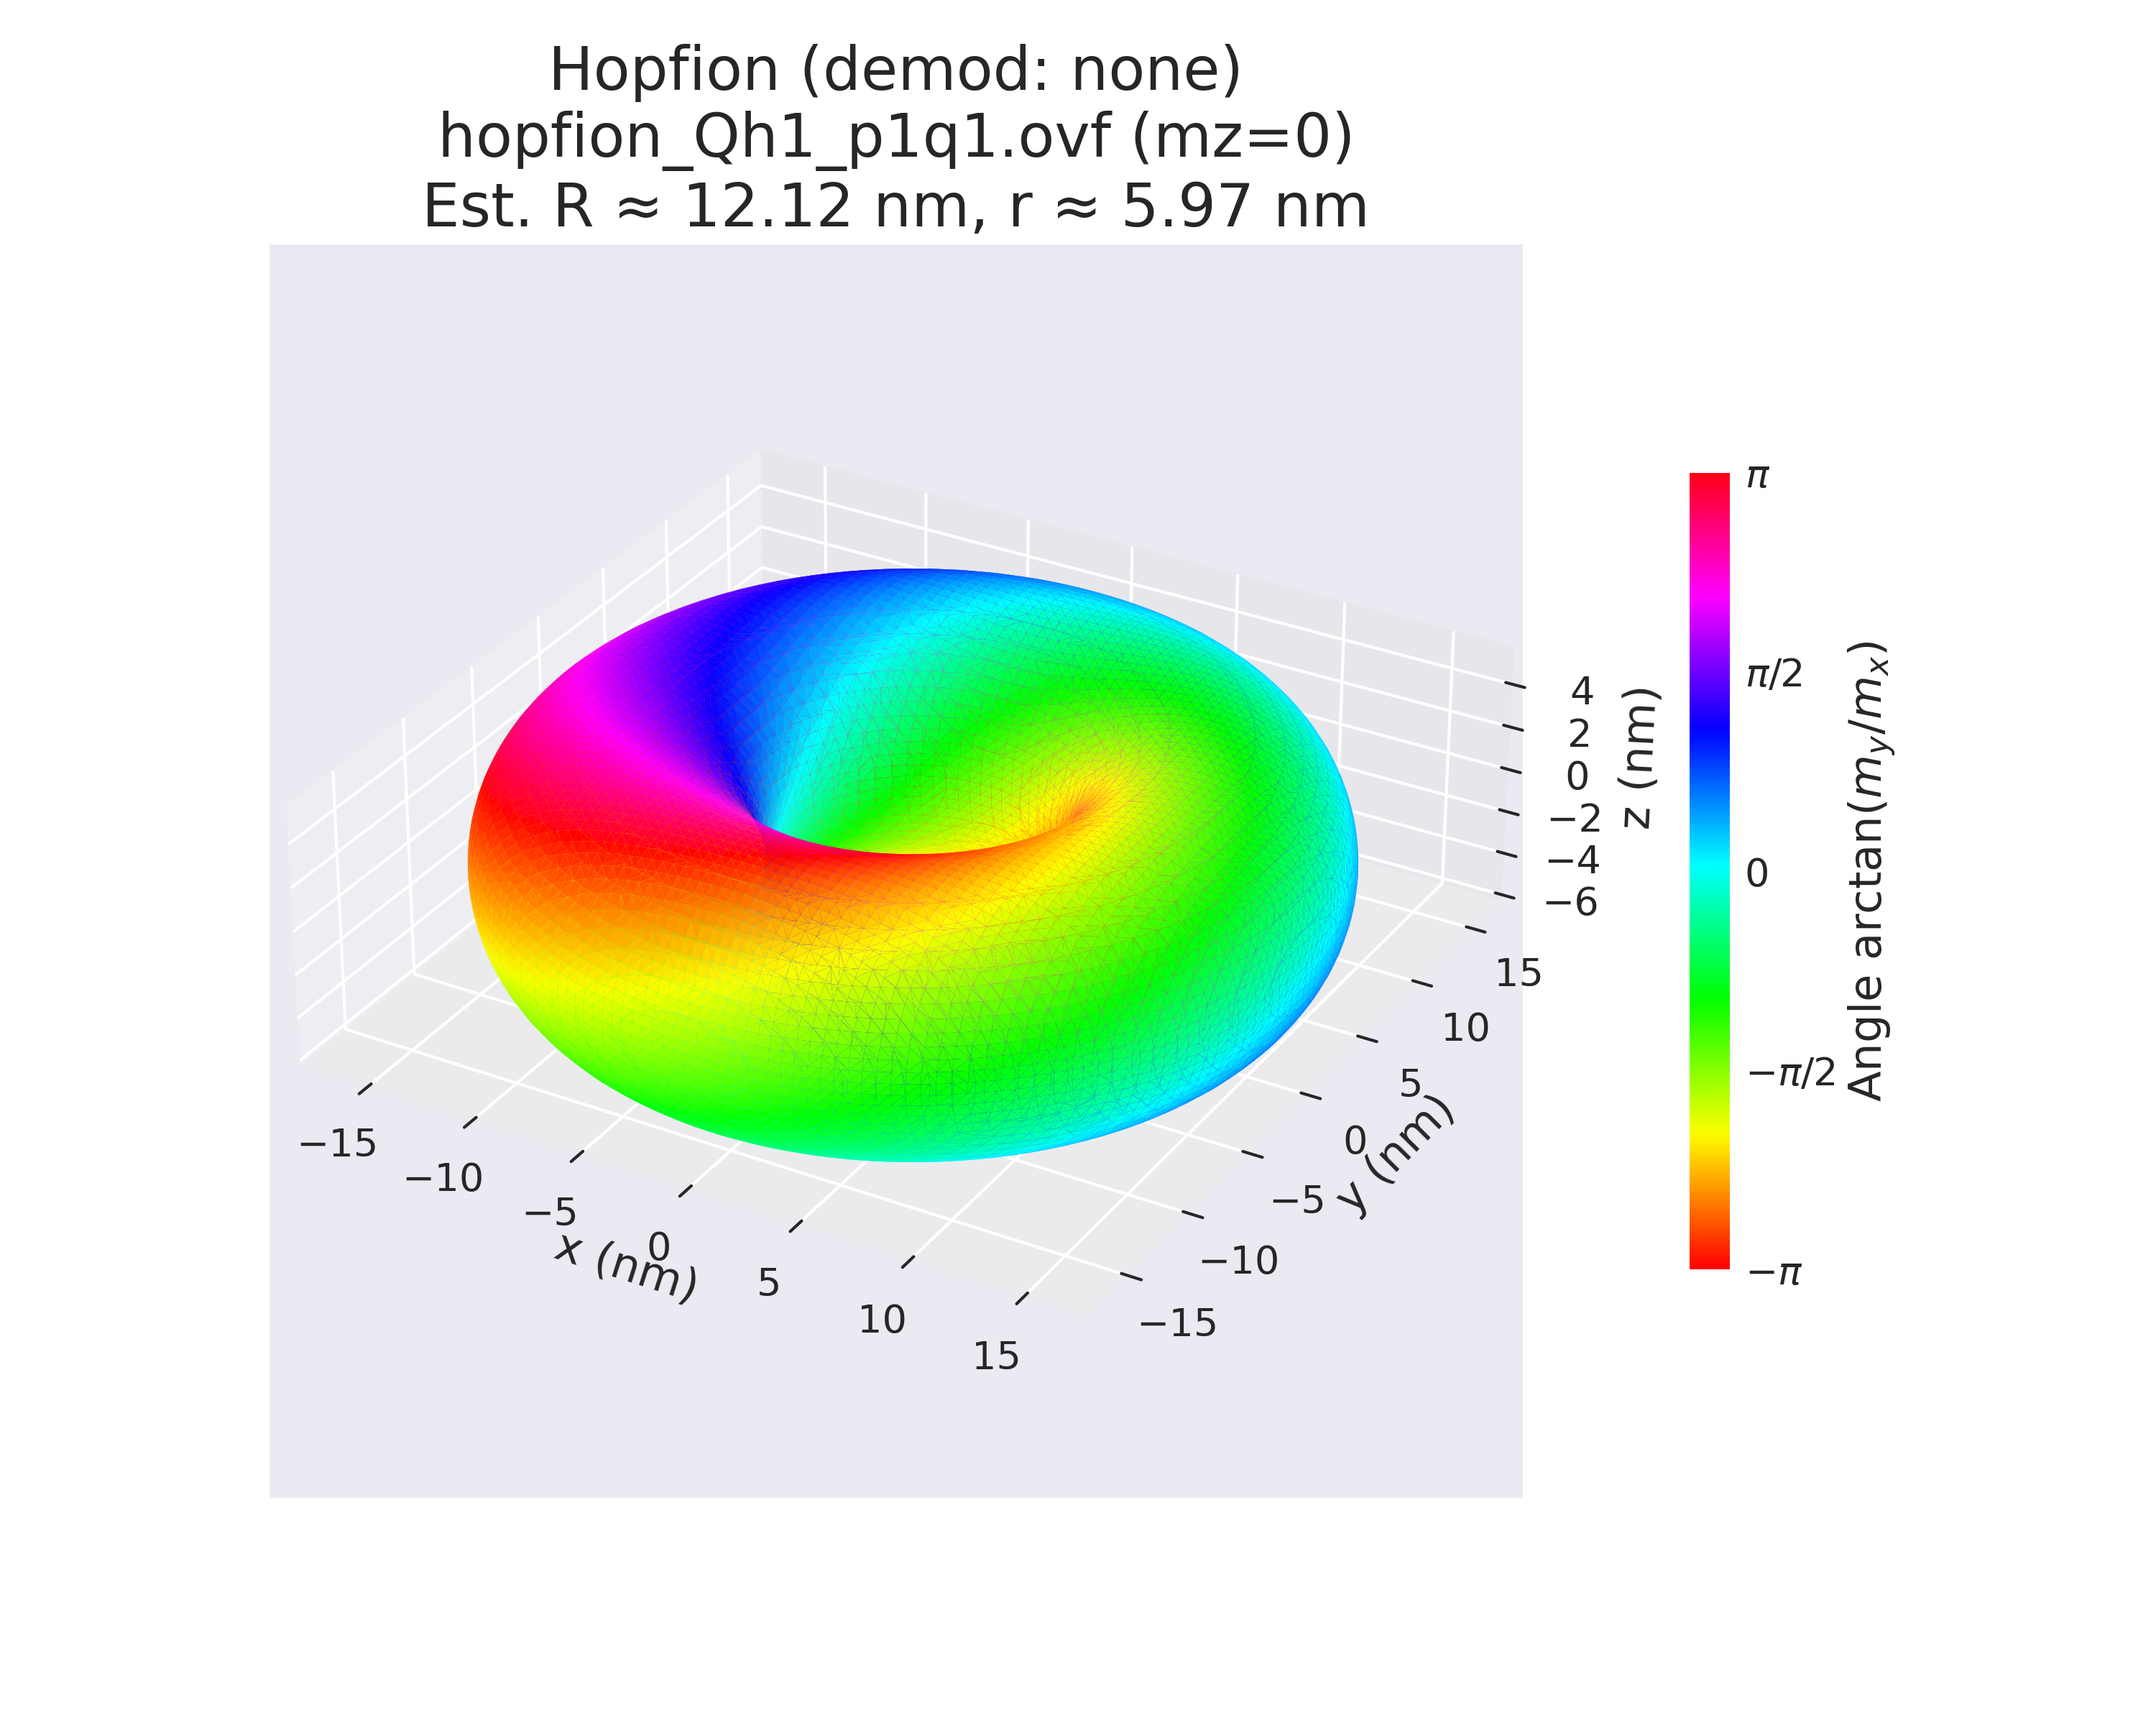
\includegraphics[width=\textwidth]{figures/hopfion_Qh1_p1q1_strategy1.png}
        \caption*{(a) $Q_H=1$ ($p=1, q=1$)}
    \end{minipage}\hfill
    \begin{minipage}{0.48\textwidth}
        \centering
        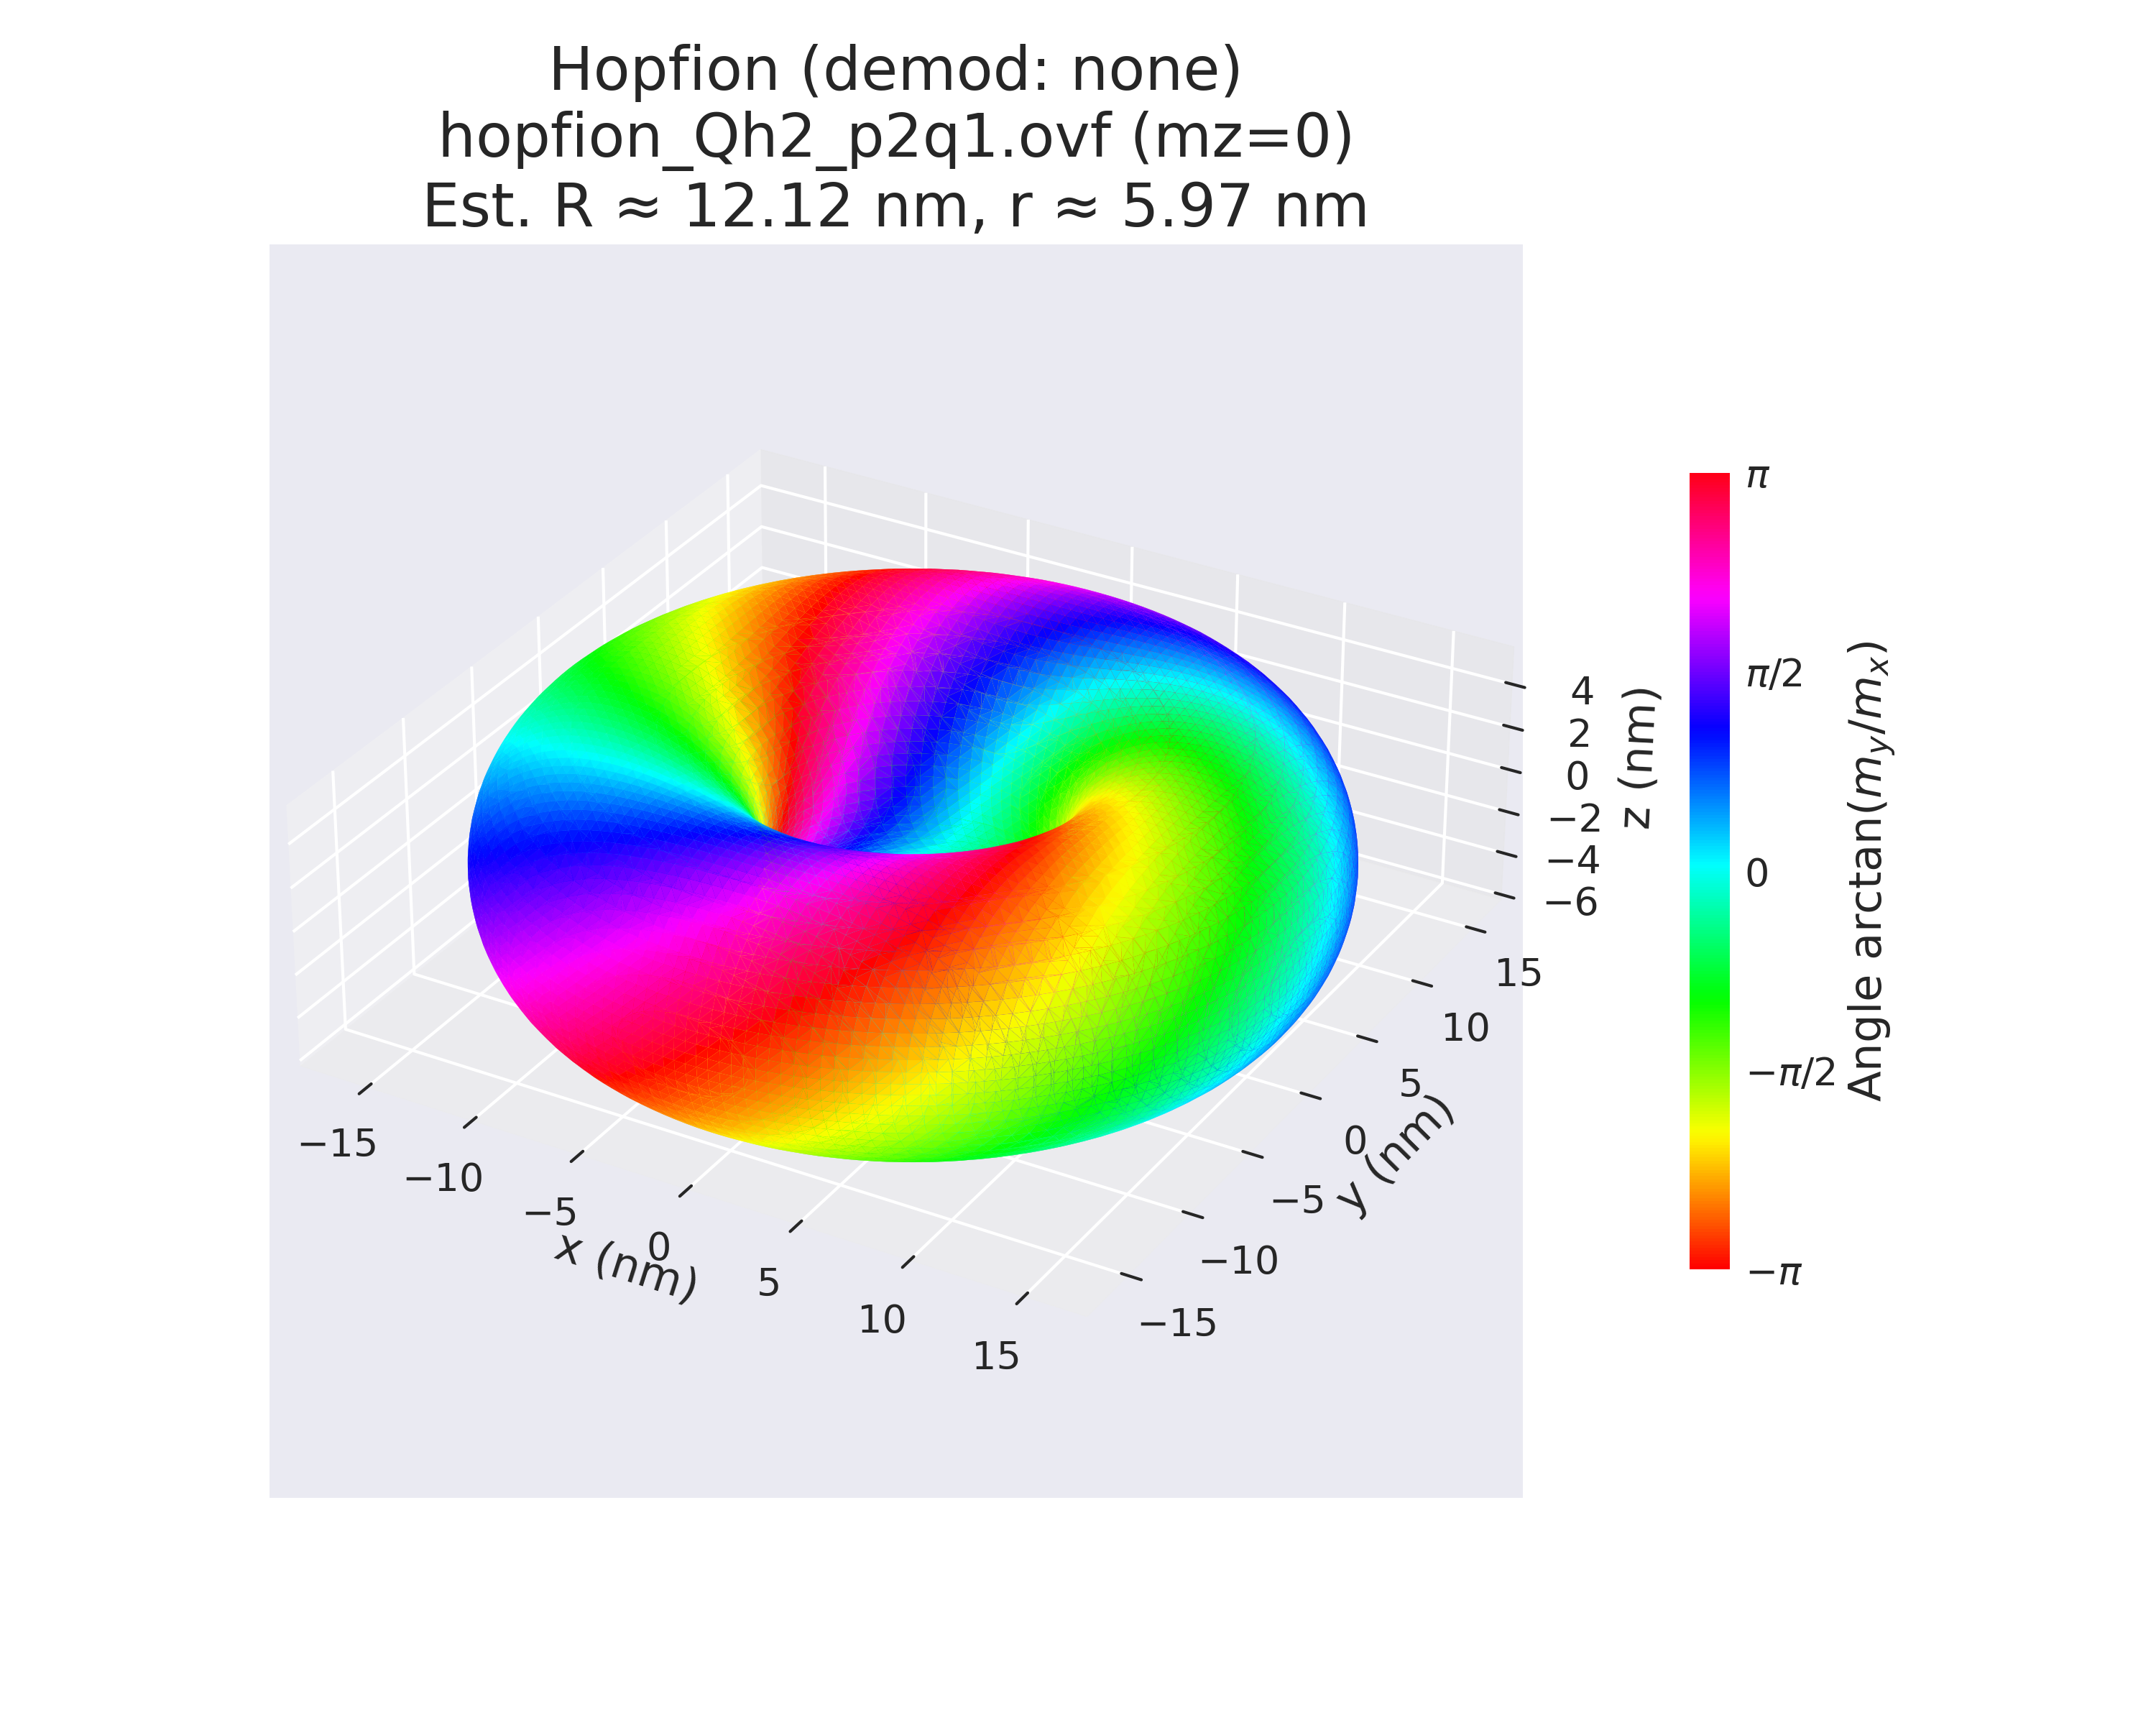
\includegraphics[width=\textwidth]{figures/hopfion_Qh2_p2q1_strategy1.png}
        \caption*{(b) $Q_H=2$ ($p=2, q=1$)}
    \end{minipage}
    
    \vspace{0.5cm}
    \begin{minipage}{0.48\textwidth}
        \centering
        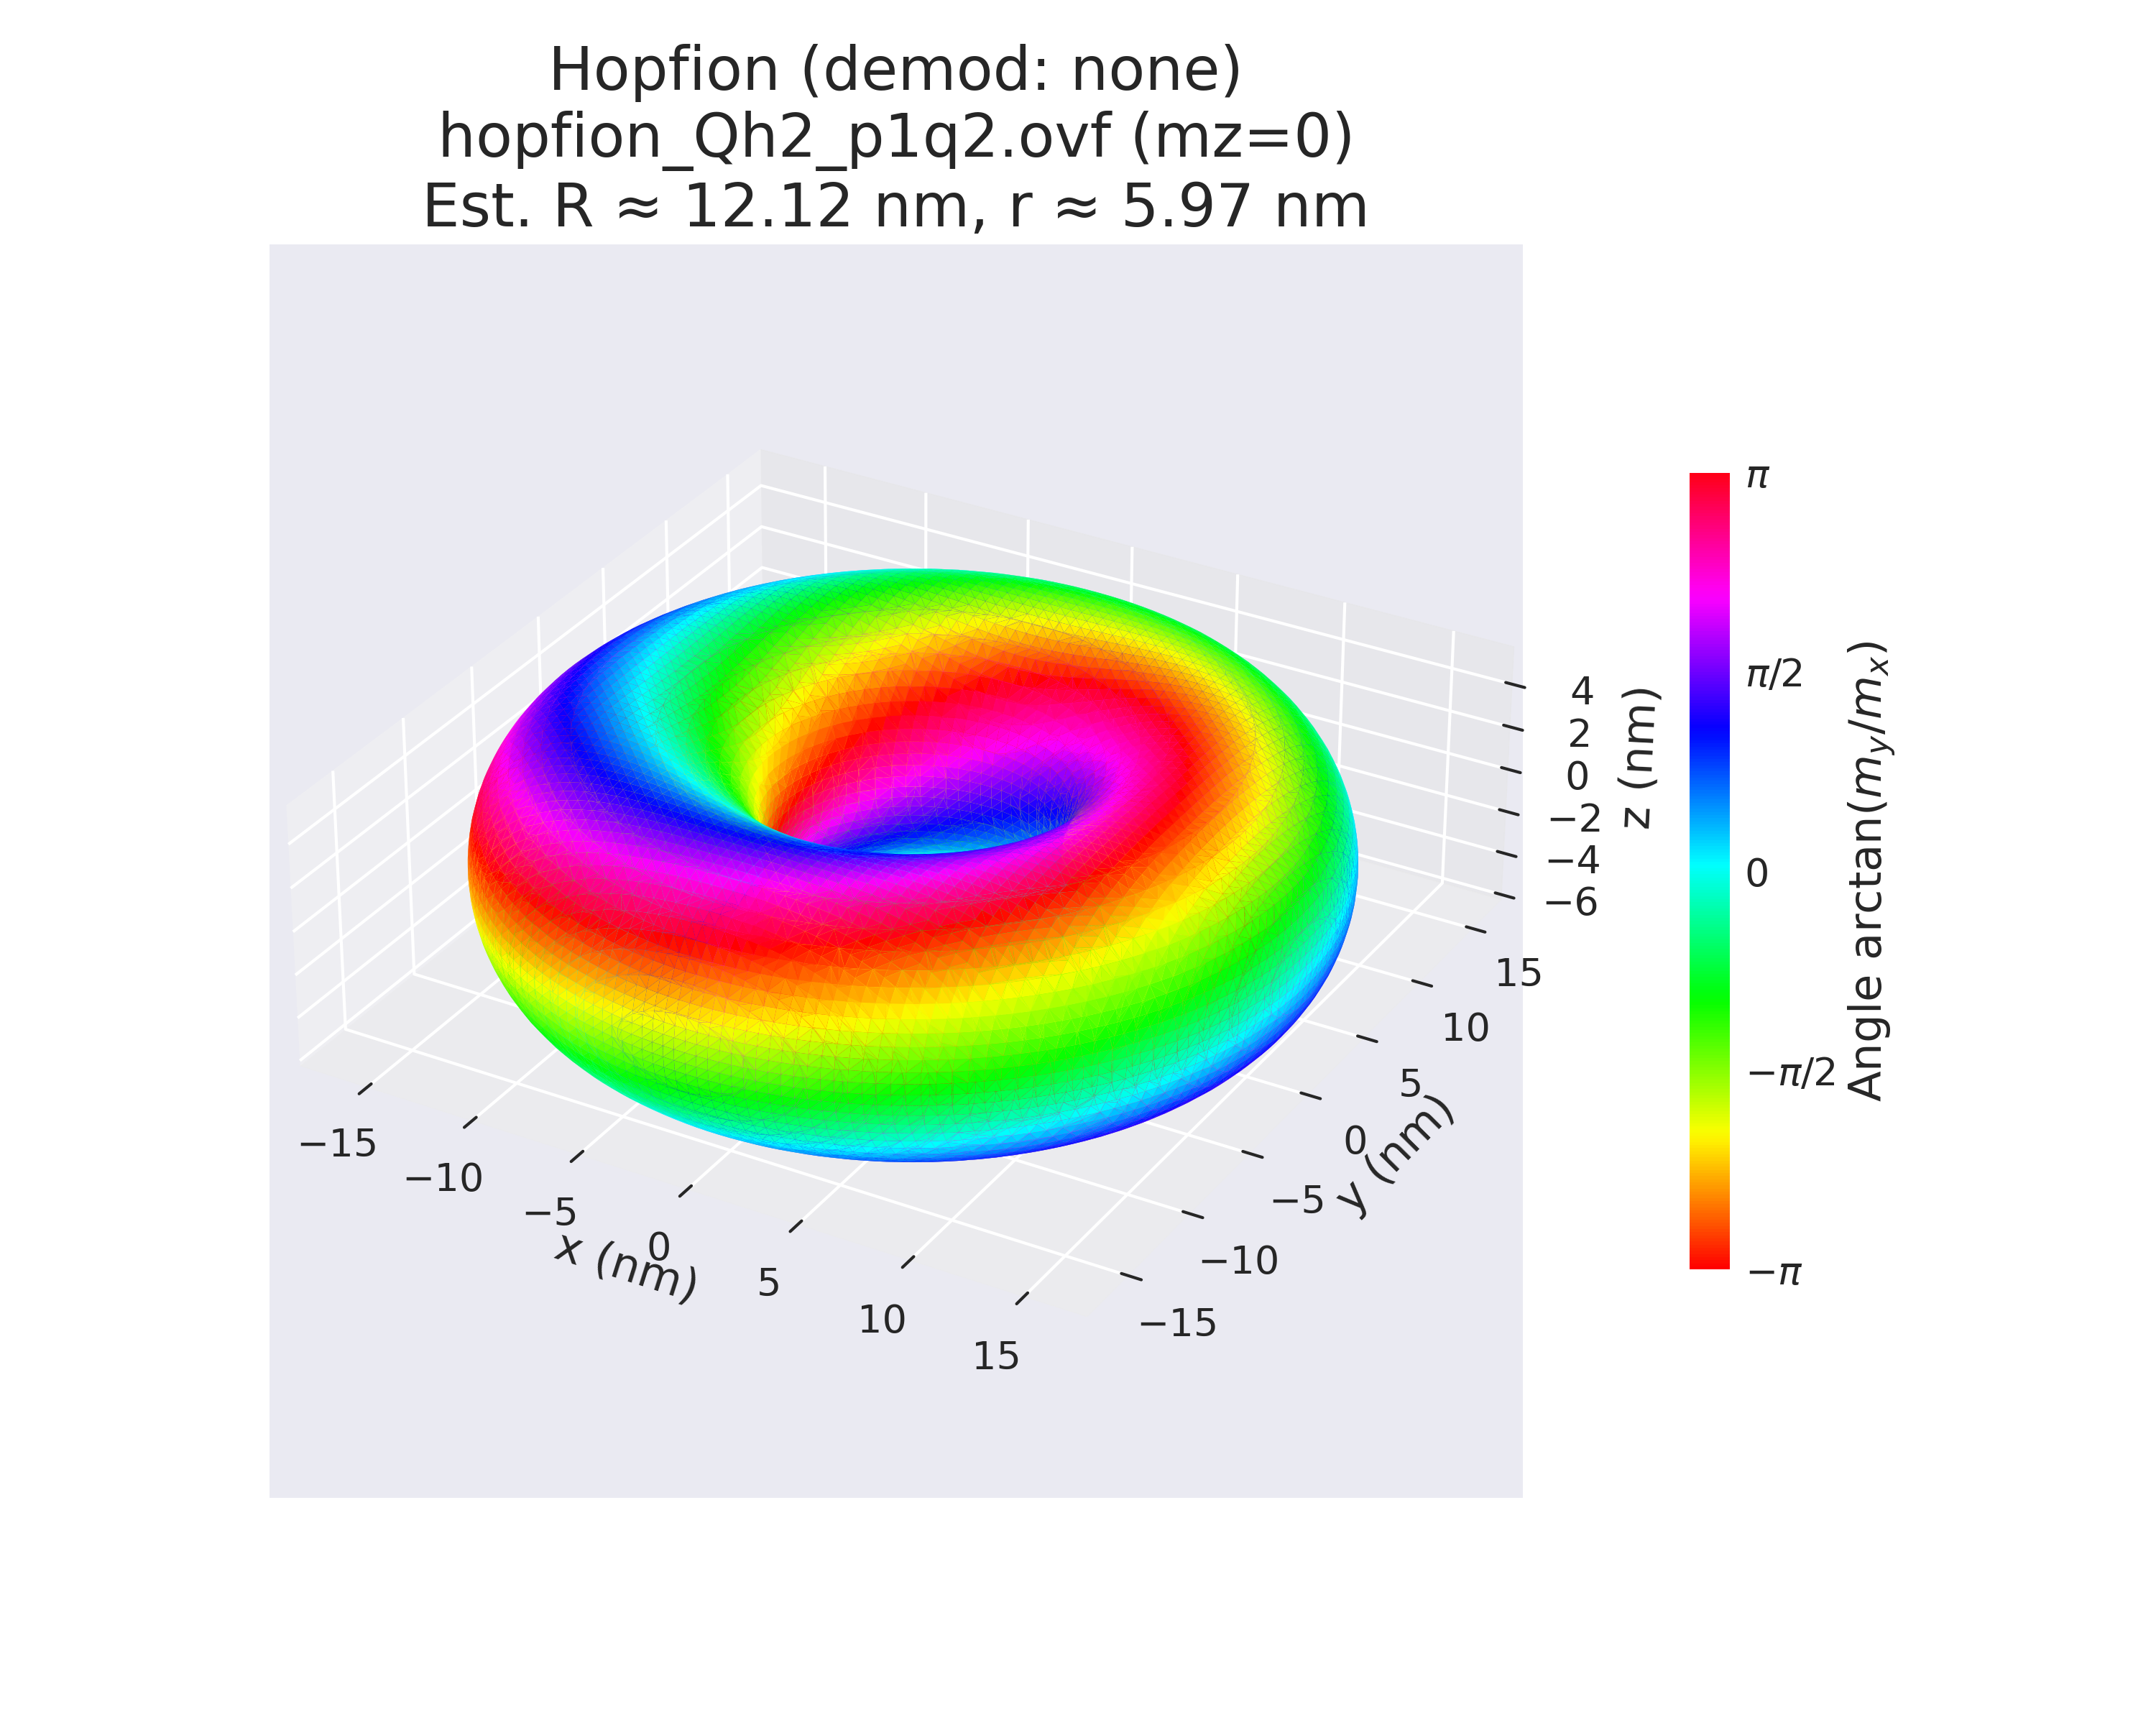
\includegraphics[width=\textwidth]{figures/hopfion_Qh2_p1q2_strategy1.png}
        \caption*{(c) $Q_H=2$ ($p=1, q=2$)}
    \end{minipage}\hfill
    \begin{minipage}{0.48\textwidth}
        \centering
        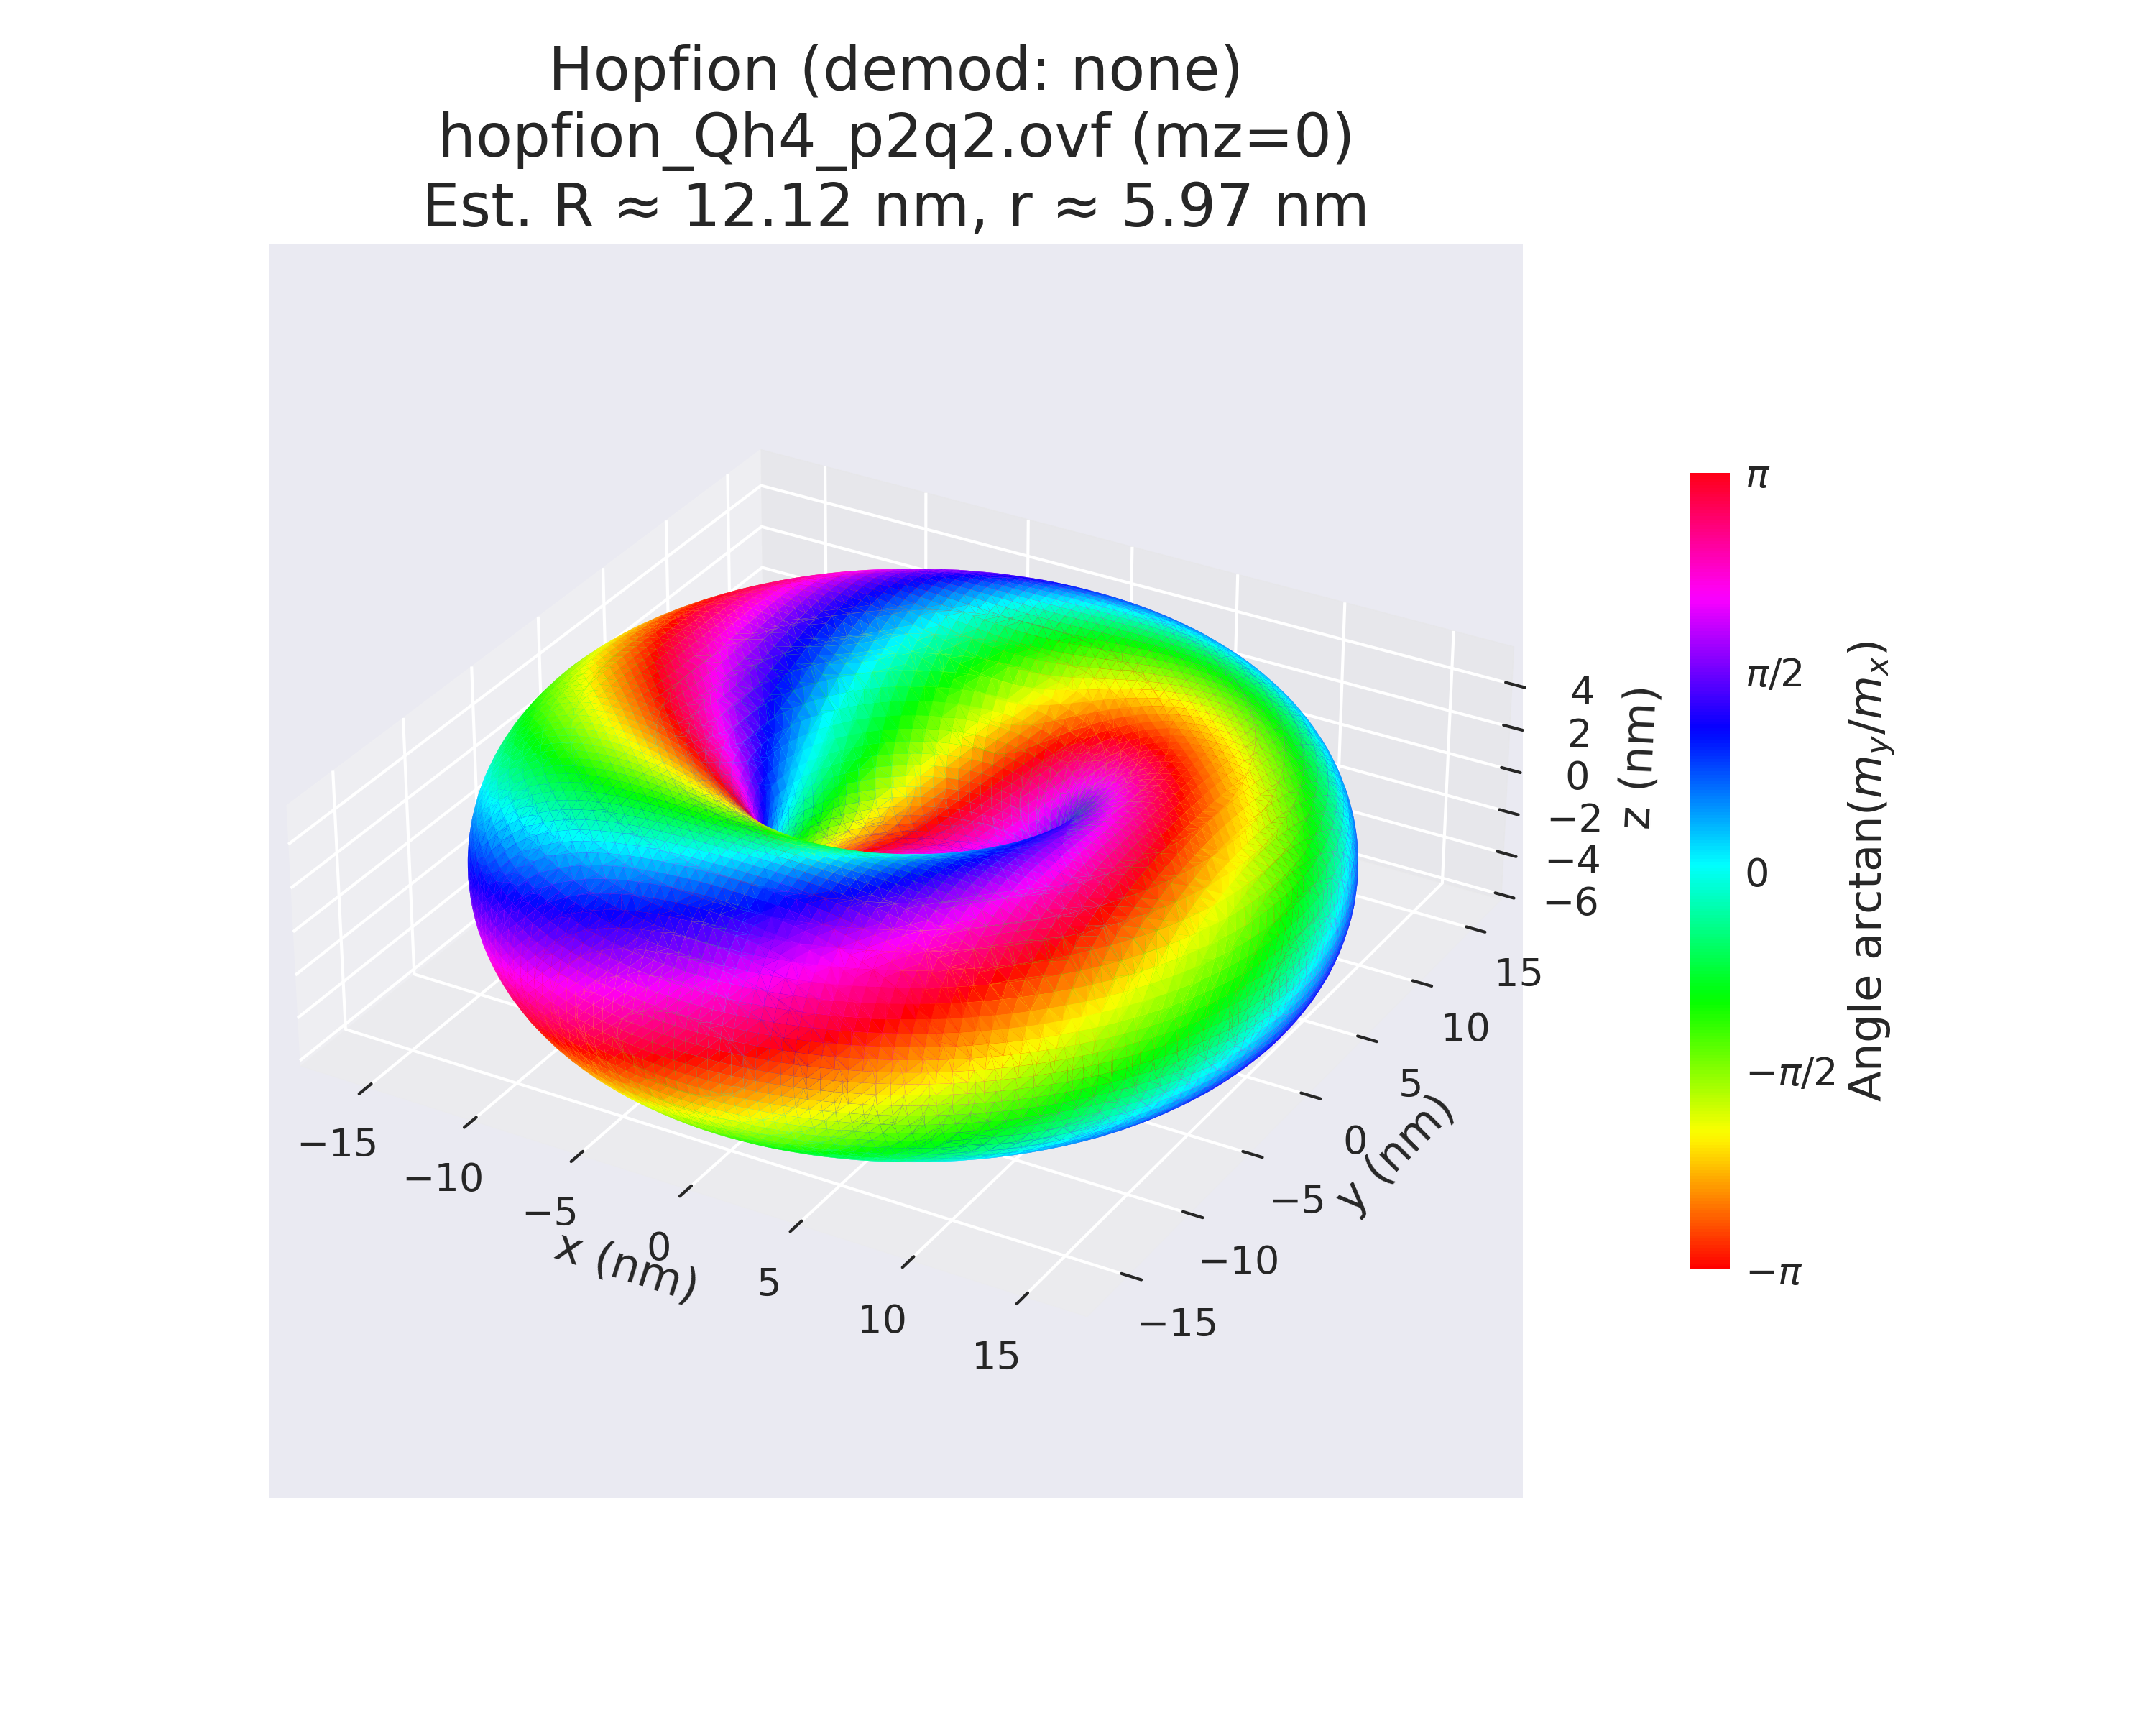
\includegraphics[width=\textwidth]{figures/hopfion_Qh4_p2q2_strategy1.png}
        \caption*{(d) $Q_H=4$ ($p=2, q=2$)}
    \end{minipage}
    \caption{使用自主离散化生成脚本构建的不同拓扑荷（$Q_H=1, 2, 4$）的 Hopfion 三维等值面及其面内相位着色对比。它们的理论特征尺寸均被设定为相同值（$R=\SI{12}{nm}, r=\SI{6}{nm}$）。}
    \label{fig:hopfion_vis}
\end{figure}

如图~\ref{fig:hopfion_vis} 所示，生成的磁化场呈现出典型的扭结拓扑结构，面内相位的颜色呈现出平滑渐变的梯度过渡，从几何形态与向量场分布双重角度验证了环面坐标理论模型及离散化构建程序的有效性。

\section{本章小结}
本章梳理了由四元数和环面坐标系描述任意拓扑荷 Hopfion 的理论框架，并基于此开发了具备坐标变换与反铁磁模式拓展功能的 OVF 初始态生成脚本。配合带 AFM 解调能力的等值面可视化算法，成功完成了模型验证。这一方法相较于传统的单一构型解析解更具普适性和灵活性，为深入研究多种类拓扑构型的稳定性及动力学行为提供了完备的初始化和分析工具。